\documentclass{purdue-slide}

% For filler text:
\usepackage[base]{babel}
\usepackage{lipsum}

\renewcommand{\titlelogo}{\includesvg[width=.3\paperwidth,keepaspectratio]{logo/cs-rev.svg}}
\renewcommand{\slidelogo}{\includesvg[width=.3\paperwidth,keepaspectratio]{logo/cs.svg}}
% For non-CS Purdue logo use the lines below:
% \renewcommand{\titlelogo}{\includesvg[width=.3\paperwidth,keepaspectratio]{logo/pu-rev.svg}}
% \renewcommand{\slidelogo}{\includesvg[width=.3\paperwidth,keepaspectratio]{logo/pu.svg}}
% You can also request a logo from https://marcom.purdue.edu/toolbox/logos/

\title{A Purdue \LaTeX\ Slide Template}
\subtitle{Made with Beamer}
\author{A Purdue Student\texorpdfstring{\footnotemark[1]}{}, A Duepur Student\texorpdfstring{\footnotemark[2]}{}}
\institute{\texorpdfstring{\footnotemark[1]}{}Purdue University, \texorpdfstring{\footnotemark[2]}{}Duepur University}
\date{Overleaf 2024 \\ Last Compiled: \today}
\renewcommand{\slidefoot}{\LaTeX\ Template}

\begin{document}

\begin{titleframe}{}
    \maketitle
\end{titleframe}

\begin{titleframe}{Text in \LaTeX}
    Examples of Basic Text Typesetting
\end{titleframe}

\section{Long Text}

\begin{frame}{This is a Really Long Text of Title Used Here}
    Some really long text:
    
    \bigskip
    
    \lipsum[2]
\end{frame}

\section{List}

\begin{frame}{Itemize List}
    Some introduction of the list.
    \begin{itemize}
        \item Bulleted copy. Keep it short with bite-size chunks of information.
        \begin{itemize}
            \item Bulleted copy. Keep it short with bite-size chunks of information.
        \end{itemize}
        \item Bulleted copy. Keep it short with bite-size chunks of information.
        \pause\item Bulleted copy on the second slide. Keep it short with bite-size chunks of information.
    \end{itemize}
\end{frame}

\begin{frame}{Enumerate List}
    Some introduction of the list.
    \begin{enumerate}
        \item Bulleted copy. Keep it short with bite-size chunks of information.
        \begin{enumerate}
            \item Bulleted copy. Keep it short with bite-size chunks of information.
        \end{enumerate}
        \item Bulleted copy. Keep it short with bite-size chunks of information.
        \item Bulleted copy. Keep it short with bite-size chunks of information.
    \end{enumerate}
\end{frame}

\begin{titleframe}{Features in \LaTeX}
    Examples of Features Commonly Used in Slides
\end{titleframe}

\section{Maths}

\begin{frame}{Maths}
    An example of some very long equations with $\Psi (x,t)$:
    
    \begin{align}
    i\hbar {\frac {\partial }{\partial t}}\Psi (x,t)&=\left[-{\frac {\hbar ^{2}}{2m}}{\frac {\partial ^{2}}{\partial x^{2}}}+V(x,t)\right]\Psi (x,t) \\
    i\hbar {\frac {d}{dt}}\vert \Psi (t)\rangle &={\hat {H}}\vert \Psi (t)\rangle \\ 
    |\Psi (t)\rangle &=\sum _{n}A_{n}e^{{-iE_{n}t}/\hbar }|\psi _{E_{n}}\rangle
    \end{align}
    
    Indeed an example of some very long equations with $\Psi (x,t)$.
\end{frame}

\section{Figure}
\begin{frame}{Figure}
    \LaTeX\ can draw figures with the tikz package:
    \begin{figure}[h]
    \centering
    \begin{tikzpicture}[
    square/.style={rectangle, draw=black!, very thick, minimum size=5mm},
    ]
    \node[square](client){\footnotesize Client};
    \node[square](r1)[right=of client]{\footnotesize Relay 1};
    \node[square](r2)[right=of r1]{\footnotesize Relay 2};
    \node[square](r3)[right=of r2]{\footnotesize Relay 3};
    \node[square](server)[right=of r3]{\footnotesize Server};
    \draw[->](client.east)--node[above=1em]{\footnotesize$E_1(E_2(E_3(P)))$}(r1.west);
    \draw[->](r1.east)--node[above=1em]{\footnotesize$E_2(E_3(P))$}(r2.west);
    \draw[->](r2.east)--node[above=1em]{\footnotesize$E_3(P)$}(r3.west);
    \draw[->](r3.east)--node[above=1em]{\footnotesize$P$}(server);
    \end{tikzpicture}
    \caption{An Example of a Three-Hop Connection}
    \label{fig:three-hop}
    \end{figure}
\end{frame}

\begin{notitleframe}
    \begin{figure}[h]
    \centering
    {
        \tikzset{font={\scriptsize\selectfont}}
        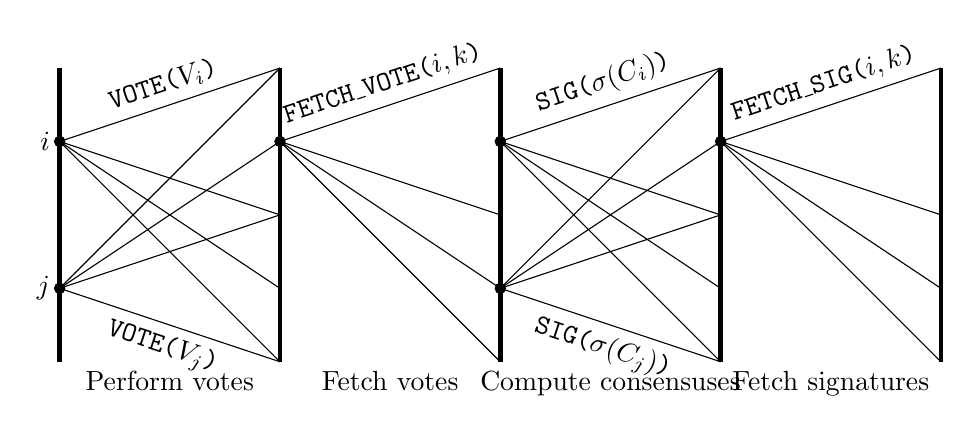
\begin{tikzpicture}[scale=\textwidth/13cm]
            \draw[black, ultra thick] (0, 0) -- (0, 4);
            \draw[black, ultra thick] (3, 0) -- (3, 4);
            \draw[black, ultra thick] (6, 0) -- (6, 4);
            \draw[black, ultra thick] (9, 0) -- (9, 4);
            \draw[black, ultra thick] (12, 0) -- (12, 4);
            \path (0, 0) -- node[anchor=north]{Perform votes} (3, 0);
            \path (3, 0) -- node[anchor=north]{Fetch votes} (6, 0);
            \path (6, 0) -- node[anchor=north]{Compute consensuses} (9, 0);
            \path (9, 0) -- node[anchor=north]{Fetch signatures} (12, 0);
            
            % Perform votes
            \filldraw[black] (0, 3) circle (2pt) node[anchor=east]{$i$};
            \filldraw[black] (0, 1) circle (2pt) node[anchor=east]{$j$};
            \draw[black] (0, 3) -- (3, 0);
            \draw[black] (0, 3) -- (3, 1);
            \draw[black] (0, 3) -- (3, 2);
            \draw[black] (0, 3) -- node[midway, above, sloped]{\texttt{VOTE($V_i$)}} (3, 4);
            \draw[black] (0, 1) -- node[midway, below, sloped]{\texttt{VOTE($V_j$)}} (3, 0);
            \draw[black] (0, 1) -- (3, 2);
            \draw[black] (0, 1) -- (3, 3);
            \draw[black] (0, 1) -- (3, 4);
            
            % Fetch votes
            \filldraw[black] (3, 3) circle (2pt);
            \draw[black] (3, 3) -- (6, 0);
            \draw[black] (3, 3) -- (6, 1);
            \draw[black] (3, 3) -- (6, 2);
            \draw[black] (3, 3) -- node[midway, above, sloped]{\texttt{FETCH\_VOTE($i, k$)}} (6, 4);
            
            % Compute consensuses
            \filldraw[black] (6, 3) circle (2pt);
            \filldraw[black] (6, 1) circle (2pt);
            \draw[black] (6, 3) -- (9, 0);
            \draw[black] (6, 3) -- (9, 1);
            \draw[black] (6, 3) -- (9, 2);
            \draw[black] (6, 3) -- node[midway, above, sloped]{\texttt{SIG($\sigma(C_i)$)}} (9, 4);
            \draw[black] (6, 1) -- node[midway, below, sloped]{\texttt{SIG($\sigma(C_j)$)}} (9, 0);
            \draw[black] (6, 1) -- (9, 2);
            \draw[black] (6, 1) -- (9, 3);
            \draw[black] (6, 1) -- (9, 4);
            
            % Fetch signatures
            \filldraw[black] (9, 3) circle (2pt);
            \draw[black] (9, 3) -- (12, 0);
            \draw[black] (9, 3) -- (12, 1);
            \draw[black] (9, 3) -- (12, 2);
            \draw[black] (9, 3) -- node[midway, above, sloped]{\texttt{FETCH\_SIG($i, k$)}} (12, 4);
            
        \end{tikzpicture}
    }
    \caption{A Large Figure}
    \label{fig:large}
    \end{figure}
    Large figures can be placed on a frame without a title.
\end{notitleframe}

\section{Block}

\begin{frame}{Block}
    Blocks emphasize information:
    \begin{block}{Block 1}
    A gold block with two different colors.
    \end{block}
    \begin{exampleblock}{Block 2}
    A gray block with two different colors.
    \end{exampleblock}
    \begin{alertblock}{Block 3}
    A red block for alert, in default theme from \LaTeX.
    \end{alertblock}
\end{frame}

\begin{titleframe}{Thank you for using!}
    For issues on the template, please visit the Github page:
    
    \texttt{https://github.com/zhtluo/purdue-slide-template}
\end{titleframe}

\end{document}